Due to time constraint, the team decided against unit testing every single component of the system. Instead, integration tests at different levels were performed.\\

\subsection{Integration testing}
The following tests were performed in the backend server by testing individual controllers, which provide the entry point of the exposed API. The tests were implemented making use of the Spring boot test module. Here we list some of them.\\

\begin{table}[H]
    \centering
    \begin{tabular}{p{3cm}p{10cm}}
    \textbf{Test ID} & INT-001-SIGN\_UP \\ \hline
    \textbf{Components} & UserController, UserService, UserRepository, Mongodb \\ \hline
    \textbf{Input} & Perform a “sign up” request. \\ \hline
    \textbf{Expected output} & “No content” response, user saved in the database. \\ \hline
    \textbf{Description} & POST request to route “/user/sign-up”. \\ \hline
    \textbf{Data used} & 
        \begin{itemize}[label={}] \itemsep0em
            \item email: test@test.com
            \item password: password
        \end{itemize} \\ \hline
    \textbf{Outcome} & Success \\ \hline
    \end{tabular}
\end{table}

\begin{table}[H]
    \centering
    \begin{tabular}{p{3cm}p{10cm}}
    \textbf{Test ID} & INT-002-GET\_CURRENT\_USER \\ \hline
    \textbf{Components} & UserController, UserService, UserRepository, Mongodb \\ \hline
    \textbf{Input} & Perform a get current user request. \\ \hline
    \textbf{Expected output} & “Ok” response with user data matching the user performing the request. \\ \hline
    \textbf{Description} & GET request to route “/user/me” with a registered user in the security context. \\ \hline
    \textbf{Outcome} & Success \\ \hline
    \end{tabular}
\end{table}

\begin{table}[H]
    \centering
    \begin{tabular}{p{3cm}p{10cm}}
    \textbf{Test ID} & INT-002-GET\_CURRENT\_USER \\ \hline
    \textbf{Components} & UserController, UserService, UserRepository, Mongodb
    \\ \hline
    \textbf{Input} & Perform a "get current user" request. \\ \hline
    \textbf{Expected output} & “Ok” response with user data matching the user performing the request. \\ \hline
    \textbf{Description} & GET request to route “/user/me” with a registered user in the security context. \\ \hline
    \textbf{Outcome} & Success \\ \hline
    \end{tabular}
\end{table}

\begin{table}[H]
    \centering
    \begin{tabular}{p{3cm}p{10cm}}
    \textbf{Test ID} & INT-003-SIGN\_IN \\ \hline
    \textbf{Components} & AuthController, AuthService, UserRepository, TokenProvider, Mongodb \\ \hline
    \textbf{Input} & Perform a “sign in” request. \\ \hline
    \textbf{Expected output} & “Ok” response with the generated JSON token. \\ \hline
    \textbf{Description} & POST request to route “/auth”. \\ \hline
    \textbf{Data used} & 
        \begin{itemize}[label={}] \itemsep0em
            \item email: user1@mail.com
            \item password: password1
        \end{itemize} \\ \hline
    \textbf{Outcome} & Success \\ \hline
    \end{tabular}
\end{table}

\begin{table}[H]
    \centering
    \begin{tabular}{p{3cm}p{10cm}}
    \textbf{Test ID} & INT-004-SIGN\_IN-WRONG\_PASSWORD \\ \hline
    \textbf{Components} & AuthController, AuthService, UserRepository, TokenProvider, Mongodb \\ \hline
    \textbf{Input} & Perform a “sign in” request with incorrect password. \\ \hline
    \textbf{Expected output} & “Unauthorized” response. \\ \hline
    \textbf{Description} & POST request to route “/auth”. \\ \hline
    \textbf{Data used} & 
        \begin{itemize}[label={}] \itemsep0em
            \item email: user1@mail.com
            \item password: wrongPassword
        \end{itemize} \\ \hline
    \textbf{Outcome} & Success \\ \hline
    \end{tabular}
\end{table}

\begin{table}[H]
    \centering
    \begin{tabular}{p{3cm}p{10cm}}
    \textbf{Test ID} & INT-005-SUBMIT\_REPORT \\ \hline
    \textbf{Components} & ViolationReportController, ViolationReportService, ViolationRepository, Mongodb \\ \hline
    \textbf{Input} & Perform a “submit report” request. \\ \hline
    \textbf{Expected output} & “Created” response. \\ \hline
    \textbf{Description} & POST request to route “/violation”. \\ \hline
    \textbf{Data used} & 
        \begin{itemize}[label={}] \itemsep0em
            \item license plate: “EX2631”
            \item description: bad parking
            \item datetime: <current time>
            \item violation type: Parking
            \item location: [9.225708, 45.479183]
        \end{itemize} \\ \hline
    \textbf{Outcome} & Success \\ \hline
    \end{tabular}
\end{table}

\begin{table}[H]
    \centering
    \begin{tabular}{p{3cm}p{10cm}}
    \textbf{Test ID} & INT-006-GET\_REPORT\_IN\_BOUNDS \\ \hline
    \textbf{Components} & ViolationReportController, ViolationReportService, ViolationRepository, Mongodb \\ \hline
    \textbf{Input} & Perform a “get reports in bounds” request. \\ \hline
    \textbf{Expected output} & “Ok” response with a list of violation reports matching the provided filters. \\ \hline
    \textbf{Description} & POST request to route “/violation/query/bounds”. \\ \hline
    \textbf{Data used} & 
        \begin{itemize}[label={}] \itemsep0em
            \item south west: [8.0, 43.0]
            \item north east: [10.0, 45.5]
            \item from: <3 hours ago>
            \item to: <current time>
            \item violation types: [Parking]
            \item violation report status: [low-confidence, high-confidence, review]
        \end{itemize} \\ \hline
    \textbf{Outcome} & Success \\ \hline
    \end{tabular}
\end{table}

\begin{table}[H]
    \centering
    \begin{tabular}{p{3cm}p{10cm}}
    \textbf{Test ID} & INT-007-GET\_API\_KEY \\ \hline
    \textbf{Components} & ApiKeyController, ApiKeyService, UserService, ApiKeyService, UserRepository, ApiKeyRepository, Mongodb \\ \hline
    \textbf{Input} & Perform a “get current user api key” request. \\ \hline
    \textbf{Expected output} & “Ok” response with the generated api key. \\ \hline
    \textbf{Description} & GET request to route “/api-key/me” with a registered user in the security context. \\ \hline
    \textbf{Outcome} & Success \\ \hline
    \end{tabular}
\end{table}

\subsection{System testing}
Complete system tests were performed in an E2E fashion, utilizing flutter\_driver to control the application running in an Android emulator, which connects to the application server. The test cases considered are the use cases defined in the RASD, following the conventional event flow, with no exceptions. This ensures the application functions as expected while maintaining a fast test suite, as E2E tests are expensive and slow compared to unit tests.\\

%system
\begin{table}[H]
    \centering
    \begin{tabular}{p{3cm}p{10cm}}
    \textbf{Test ID} & SYS-001-SIGN\_UP \\ \hline
    \textbf{Input} & Perform a sign up through the application. \\ \hline
    \textbf{Expected output} & Successful sign in with the new user created, redirecting to home screen. \\ \hline
    \textbf{Description} & While on the sign in screen, press the “sign up” button which redirects to the sign up screen where the form is filled and submitted. Once redirected to the sign in screen, fill the form with the new users email and password and submit it. Check that the application redirects to the home screen. \\ \hline
    \textbf{Data used} & 
        \begin{itemize}[label={}] \itemsep0em
            \item email: email@mail.com
            \item password: password
            \item name: name
            \item surname: surname
            \item username: username
        \end{itemize} \\ \hline
    \textbf{Outcome} & Success \\ \hline
    \end{tabular}
\end{table}

\begin{table}[H]
    \centering
    \begin{tabular}{p{3cm}p{10cm}}
    \textbf{Test ID} & SYS-002-SIGN\_IN \\ \hline
    \textbf{Input} & Perform a sign in through the application. \\ \hline
    \textbf{Expected output} & Successful sign in with an already created user, redirecting to the home screen. \\ \hline
    \textbf{Description} & While on the sign in screen, fill the form with email and password of an existing user in the database. Then check that the application redirects to the home screen. \\ \hline
    \textbf{Data used} & 
        \begin{itemize}[label={}] \itemsep0em
            \item email: user0@mail.com
            \item password: password1
        \end{itemize} \\ \hline
    \textbf{Outcome} & Success \\ \hline
    \end{tabular}
\end{table}

\begin{table}[H]
    \centering
    \begin{tabular}{p{3cm}p{10cm}}
    \textbf{Test ID} & SYS-003-SHOW\_PROFILE \\ \hline
    \textbf{Input} & Enter profile screen. \\ \hline
    \textbf{Expected output} & Correct data displayed in the profile screen. \\ \hline
    \textbf{Description} & While on the home screen, navigate to the profile screen. Check that the information displayed matches the one stored in the database. \\ \hline
    \textbf{Outcome} & Success \\ \hline
    \end{tabular}
\end{table}

\begin{table}[H]
    \centering
    \begin{tabular}{p{3cm}p{10cm}}
    \textbf{Test ID} & SYS-004-OBTAIN\_API\_KEY \\ \hline
    \textbf{Input} & Tap “get API key”. \\ \hline
    \textbf{Expected output} & API key shown on screen. \\ \hline
    \textbf{Description} & While on the profile screen, tap the “get API key” button. Wait for an API key to be displayed. \\ \hline
    \textbf{Outcome} & Partial success (see note). \\ \hline
    \textbf{Note} & Due to a limitation of the framework, the widget used to show text that is also selectable (so the user can copy the key) cannot be read with the test driver, so the key cannot be compared to make sure its the same as a predefined value. Only the presence of a key is checked. \\ \hline
    \end{tabular}
\end{table}

\begin{table}[H]
    \centering
    \begin{tabular}{p{3cm}p{10cm}}
    \textbf{Test ID} & SYS-005-EDIT\_PROFILE \\ \hline
    \textbf{Input} & Edit the user profile. \\ \hline
    \textbf{Expected output} & New profile information shown on profile page. \\ \hline
    \textbf{Description} & While on the profile screen, tap the “edit” button which redirects to the edit profile screen. There, fill the form with new information and submit it. This redirects to the profile screen, where the profile information is checked. \\ \hline
    \textbf{Data used} & 
        \begin{itemize}[label={}] \itemsep0em
            \item name: newName
            \item surname: newSurname
            \item username: newUsername
            \item email: newMail@mail.com
        \end{itemize} \\ \hline
    \textbf{Outcome} & Success \\ \hline
    \end{tabular}
\end{table}

\begin{table}[H]
    \centering
    \begin{tabular}{p{3cm}p{10cm}}
    \textbf{Test ID} & SYS-006-SIGN\_OUT \\ \hline
    \textbf{Input} & Perform a sign out. \\ \hline
    \textbf{Expected output} & Application redirects to the login screen. \\ \hline
    \textbf{Description} & While on the profile screen, press the “sign out” button, then check that the application redirects to the sign out screen. \\ \hline
    \textbf{Outcome} & Success \\ \hline
    \end{tabular}
\end{table}

\begin{table}[H]
    \centering
    \begin{tabular}{p{3cm}p{10cm}}
    \textbf{Test ID} & SYS-007-SUBMIT\_REVIEW \\ \hline
    \textbf{Input} & Perform a report review. \\ \hline
    \textbf{Expected output} & Review submitted successfully. \\ \hline
    \textbf{Description} & While on the home screen with a user with a review request, tap the review notification button. An alert is shown with a license plate field where a license plate is inputted and submitted. Once the alert closes, check that a message is displayed indicating a successful review. \\ \hline
    \textbf{Data used} & 
        \begin{itemize}[label={}] \itemsep0em
            \item Logged in as:
            \begin{itemize}[label={}] \itemsep0em
                \item email: user0@mail.com
                \item password: password1
            \end{itemize}
            \item License plate: EX215GC
        \end{itemize} \\ \hline
    \textbf{Outcome} & Success \\ \hline
    \end{tabular}
\end{table}

\begin{table}[H]
    \centering
    \begin{tabular}{p{3cm}p{10cm}}
    \textbf{Test ID} & SYS-008-SUBMIT\_REPORT \\ \hline
    \textbf{Input} & Submit a violation report. \\ \hline
    \textbf{Expected output} & Report submitted successfully. \\ \hline
    \textbf{Description} & While on the home screen press the “Submit a report” card, which redirects to the violation report screen. Once there, fill the form, press the take a photo button, which automatically loads a mocked car picture and press confirm. On the alert to confirm the license plate photo press ok. Check that a message is displayed indicating a successful submission and the application redirects to the home screen. \\ \hline
    \textbf{Data used} & 
        \begin{itemize}[label={}] \itemsep0em
            \item violation type: Parking
            \item license plate: DX034PS
            \item description: testing
            \item photo: 
            \item 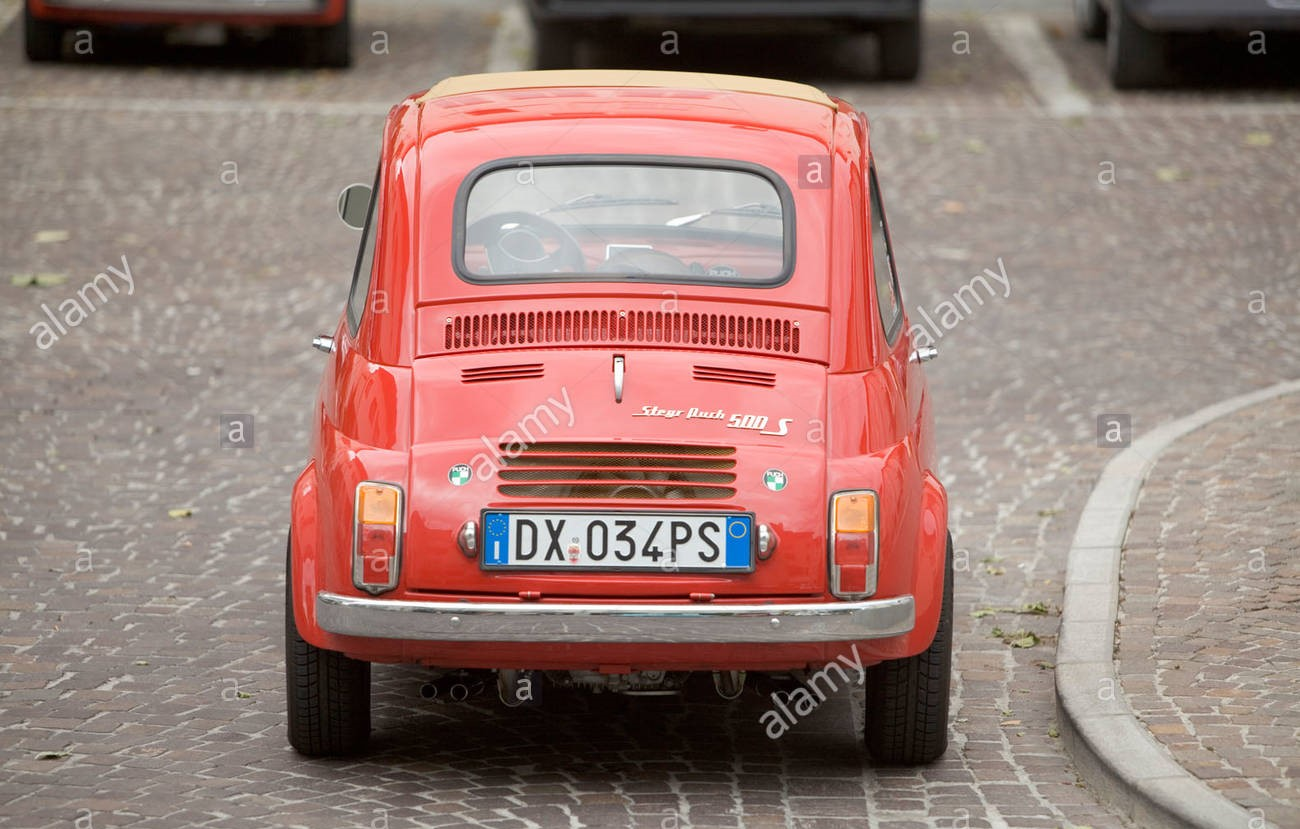
\includegraphics[width=.3\textwidth]{Images/test-photo.jpg}
        \end{itemize} \\ \hline
    \textbf{Outcome} & Success \\ \hline
    \end{tabular}
\end{table}

\begin{table}[H]
    \centering
    \begin{tabular}{p{3cm}p{10cm}}
    \textbf{Test ID} & SYS-009-SHOW\_REPORTS\_MAP \\ \hline
    \textbf{Input} & Go to map screen. \\ \hline
    \textbf{Expected output} & Report marker shown on the map. \\ \hline
    \textbf{Description} & Repeat the procedure for Test SYS-008-SUBMIT\_REPORT in order to have a report on the current location. On the home screen, tap the “Reports map” card. Once redirected to the map screen, check that there is a report marker visible on the map. \\ \hline
    \textbf{Outcome} & Partial success (see note) \\ \hline
    \textbf{Note} & Due to limitations of the framework, the filter functionality could not be tested. \\ \hline
    \end{tabular}
\end{table}


% \begin{table}[H]
%     \centering
%     \begin{tabular}{p{3cm}p{10cm}}
%     \textbf{Test ID} & aaaa \\ \hline
%     \textbf{Input} & aaaa \\ \hline
%     \textbf{Expected output} & aaaa \\ \hline
%     \textbf{Description} & aaaa \\ \hline
%     \textbf{Data used} & 
%         \begin{itemize}[label={}] \itemsep0em
%             \item aaaa
%             \item aaaa
%             \item aaaa
%             \item aaaa
%             \item aaaa
%         \end{itemize} \\ \hline
%     \textbf{Outcome} & Success \\ \hline
%     \end{tabular}
% \end{table}